 


\documentclass[journal]{IEEEtran}
 


% correct bad hyphenation here
\hyphenation{op-tical net-works semi-conduc-tor
\usepackage{float}
\usepackage{graphicx}
\usepackage{algorithm}
\usepackage{algorithmic}
\usepackage{amsmath}
\usepackage{color}

\usepackage{soul}


\begin{document}
% Start with \small to reduce font size globally
\small
%
% paper title
% Titles are generally capitalized except for words such as a, an, and, as,
% at, but, by, for, in, nor, of, on, or, the, to and up, which are usually
% not capitalized unless they are the first or last word of the title.
% Linebreaks \\ can be used within to get better formatting as desired.
% Do not put math or special symbols in the title.
\title{Optimizing Content Cache with Vehicular Edge Computing: A Deep Federated Learning based Novel Predictive Study}

\author{Azan Ali Khan, Basharat Hussain\textsuperscript{*}, Muhammad Islam

 \thanks{Azan A K is perusing his MS degree in Computer Science, FAST University (NUCES), Islamabad 44000, Pakistan (email: i222938@nu.edu.pk)} 
 \thanks{Hussain B is working with the Department of Computer Science, FAST University (NUCES), Islamabad 44000, Pakistan}
 \thanks{Mumhammad I is working with the College of Sci. \& Eng., James Cook Univ., Cairns, QLD, Australia (email: muhammad.islam1@my.jcu.edu.au)} 
  \thanks{Maryam M A D is working with Department of CS\&E, College of CS\&E, University of Hafr Al Batin, KSA (email: maldabel@uhb.edu.sa)} 
   \thanks{Ali K B is working with the Department of Computing and Mathematics, Manchester Metropolitan University, Manchester, U.K. (email: dr.alikashif.b@ieee.org)} 
\thanks{\textsuperscript{*} Correspondence: basharat.hussain@isb.nu.edu.pk}
}


% The paper headers
\markboth{}%
{Hussain \MakeLowercase{\textit{et al.}}: A Sample Article Using IEEEtran.cls for IEEE Journals}
\maketitle

%
% author names and IEEE memberships
% note positions of commas and nonbreaking spaces ( ~ ) LaTeX will not break
% a structure at a ~ so this keeps an author's name from being broken across
% two lines.
% use \thanks{} to gain access to the first footnote area
% a separate \thanks must be used for each paragraph as LaTeX2e's \thanks
% was not built to handle multiple paragraphs



% note the % following the last \IEEEmembership and also \thanks - 
% these prevent an unwanted space from occurring between the last author name
% and the end of the author line. i.e., if you had this:
% 
% \author{....lastname \thanks{...} \thanks{...} }
%                     ^------------^------------^----Do not want these spaces!
%
% a space would be appended to the last name and could cause every name on that
% line to be shifted left slightly. This is one of those "LaTeX things". For
% instance, "\textbf{A} \textbf{B}" will typeset as "A B" not "AB". To get
% "AB" then you have to do: "\textbf{A}\textbf{B}"
% \thanks is no different in this regard, so shield the last } of each \thanks
% that ends a line with a % and do not let a space in before the next \thanks.
% Spaces after \IEEEmembership other than the last one are OK (and needed) as
% you are supposed to have spaces between the names. For what it is worth,
% this is a minor point as most people would not even notice if the said evil
% space somehow managed to creep in.








% If you want to put a publisher's ID mark on the page you can do it like
% this:
%\IEEEpubid{0000--0000/00\$00.00~\copyright~2015 IEEE}
% Remember, if you use this you must call \IEEEpubidadjcol in the second
% column for its text to clear the IEEEpubid mark.



% use for special paper notices
%\IEEEspecialpapernotice{(Invited Paper)}




% make the title area
\maketitle

% As a general rule, do not put math, special symbols or citations
% in the abstract or keywords.
\begin{abstract}
This paper proposes an innovative framework for enhancing vehicular edge
computing (VEC) efficiency by addressing challenges in traditional intelligent transportation systems and internet of vehicles. Our aim is to improve
content prediction accuracy, reduce offload latency, and ensure data privacy by utilizing advanced techniques such as federated learning (FL) and deep reinforcement learning. We propose an in-car popularity-based caching (PBC) asynchronous system, based on FL,  for edge computing. Unlike traditional synchronous FL, asynchronous FL allows the global model to be updated without waiting for all cars to complete learning process and upload their individual models, which helps to reduce training time. Integrating VEC with roadside infrastructure system allows real-time data processing by enabling low latency and high-quality services for applications like traffic management and autonomous driving. Through collaborative caching schemes and personalized content delivery, the proposed model optimizes system performance while adapting to dynamic vehicular environments. By prefetching potentially popular content ahead of time and caching it in edge nodes or roadside units, depending on the position and movement direction of the vehicle, the PBC system reduces the delay in content queries. Comprehensive experimental evaluations demonstrate that the PBC technique outperforms existing benchmark caching schemes in reducing the latency.   
\end{abstract}

% Note that keywords are not normally used for peerreview papers.
\begin{IEEEkeywords} Federated learning, Vehicular edge computing, Intelligent transportation, Federated learning, Variational autoencoders, Federated vehicular networks, Internet of vehicles, Mobile edge computing, Double dueling deep Q-networ, Popularity-based caching.
\end{IEEEkeywords}






% For peer review papers, you can put extra information on the cover
% page as needed:
% \ifCLASSOPTIONpeerreview
% \begin{center} \bfseries EDICS Category: 3-BBND \end{center}
% \fi
%
% For peerreview papers, this IEEEtran command inserts a page break and
% creates the second title. It will be ignored for other modes.
\IEEEpeerreviewmaketitle

\section{Introduction}
% The very first letter is a 2 line initial drop letter followed
% by the rest of the first word in caps.
% 
% form to use if the first word consists of a single letter:
% \IEEEPARstart{A}{demo} file is ....
% 
% form to use if you need the single drop letter followed by
% normal text (unknown if ever used by the IEEE):
% \IEEEPARstart{A}{}demo file is ....
% 
% Some journals put the first two words in caps:
% \IEEEPARstart{T}{his demo} file is ....
% 
% Here we have the typical use of a "T" for an initial drop letter
% and "HIS" in caps to complete the first word.
\IEEEPARstart{I}{ntelligent} transportation systems (ITS) \cite{r2_its} and the Internet of vehicles (IOV) \cite{r2_iov} are vital components of future smart cities, providing accurate and real-time traffic monitoring to help authorities stay informed about constantly changing traffic conditions. Traditional ITS and IOV systems face several challenges, including high offload latency and inaccuracies in caching and content prediction techniques. Furthermore, the issue of poor service quality caused by vehicle movement must be resolved. 
These difficulties can hinder the delivery of high-quality and low-latency services in automotive environments.
In vehicular networking, data security and privacy issues must be addressed, while also considering how vehicle movement impacts model updates and communication protocols. We used cutting-edge methods like deep reinforcement learning (DRL) \cite{r2_drl}, (FL) \cite{r2_fl} with optimization techniques to solve these problems. These methods reduce latency, improve content prediction and caching accuracy, and safeguard vehicle privacy. 

VEC integrates edge computing technology into vehicle networks, aiming to use edge servers at roadside units (RSUs) to support in-vehicle applications \cite{r2_vanet}. Driven by advancements in wireless communication, edge computing enables real-time data processing and decision-making at the edge of the network. VEC enables low-latency and high-quality services by offloading computational tasks and caching content closer to the vehicles. VEC, therefore, holds significant promise for transforming transportation systems and enabling a variety of innovative applications. 
% In VEC, vehicles use onboard computing and wireless communication to access network edge resources, enabling low-latency applications like traffic management and autonomous driving. 
Key challenges, in VEC, include vehicle mobility, limited processing power, and ensuring data privacy and security.
While vehicles move through urban areas, their data requests change quickly, requiring efficient caching and prediction to reduce latency and improve service quality. Prefetching and caching popular content at edge nodes address this need. However, traditional methods struggle in VEC environments due to complex vehicle mobility, limited computing power, and the challenge of protecting user privacy. 
As a potential solution to these issues, FL enables collaborative model training across dispersed devices while maintaining data privacy. In this context, this research proposal aims to develop a novel framework by utilizing an innovative caching scheme. Such scheme combines FL, DRL, and a variational autoencoder specifically tailored for cloud-based edge computing. Using the collective intelligence of vehicles and road infrastructure in the proposed model, we further build a superior personalized model that is powered by caching efficiency.

The motivation for this research stems from an efficient vehicular edge computing by addressing the challenges faced by traditional ITS and IOV systems, such as poor accuracy in content prediction, high offload latency, and data privacy concerns. A typical VEC system is illustrated in Fig. \ref{fig:vec_system} where a generic VEC system is presented that integrates edge nodes (RSUs and servers) and vehicles for low-latency, high-bandwidth processing, enhancing autonomous driving, traffic management services. Current methods face challenges due to the limited computational power within vehicles, leading to prolonged training times for local models and impacting the accuracy of cache hit rate predictions.
The aim is to enhance the efficiency of in-vehicle applications by leveraging advanced technologies like FL and DRL to optimize content caching strategies in VEC. We desire to enhance the global models' accuracy employed in VEC by incorporating mobile features like position, direction and speed of the vehicle. 
% We aim to design a collaborative caching scheme to (a) optimize  content delivery speed by reducing latency, (b) predict popular content efficiently, and (c) provide personalized services to vehicular users (VUs) while adapting to dynamic mobility environment. 
The significant contributions in this research work are:\para 
\begin{enumerate}
\item \textit{Enhancing global model accuracy:} To improve the global models' accuracy, we present an deep FL framework that incorporates vehicle mobility characteristics, such as position and speed. By adapting the training process to reflect these mobility factors, we create a more robust global model for VEC environments.


\item \textit{Caching:} We suggest a technique where a global model is applied to capture popular content using a \textit{variational autoencoder} (VAE), and the RSU stores the popular content of all cars in its coverage area.


\item \textit{DRL framework:} To address the caching problem in vehicular edge computing, we propose a deep reinforcement learning framework utilizing a \textit{dueling double deep Q-network }(DDQN). This model allows each RSU to identify the best caching strategies that reduce content transmission delays by specifying the state, action, and reward functions. This model utilizes vehicle and RSU-level data to improve decision-making, leading to a more efficient content delivery system.
\end{enumerate}

\section{Related Work}
Over the past decade, researchers have focused on exploring vehicular networks by using FL, a technique that enables vehicles to train local models using their own data and subsequently upload these models to RSUs to update a shared global model. These methodologies ensure the protection of private information while establishing an efficient caching scheme in VEC. 
% Numerous studies have explored FL-based caching strategies within the VEC domain. 
Several studies have emphasized the importance of optimizing energy-efficient resources in FL for vehicular networks. The authors in \cite{Xiao2022-zg} underscore the significance of resource and delay optimization in FL, particularly in real-time scenarios like autonomous driving. Their approach aims to balance learning time, energy consumption, and system performance dynamically, thus optimizing resource allocation. Similarly, Jing et al. \cite{Wu2021-ux} introduce a framework for V2E communications that optimizes resource allocation to reduce energy consumption and enhance network performance.\par
Addressing the challenges associated with high system costs in edge caching within vehicular networks, some researchers propose mobility-aware coded edge caching strategies leveraging deep reinforcement learning \cite{r3}. By optimizing caching decisions considering vehicle mobility and dynamic content popularity, these approaches aim to minimize system costs while improving network performance. The research work in  \cite{r4} introduces a selective model aggregation approach within FL to enhance efficiency and accuracy. By leveraging contract-based selection processes and a greedy algorithm, their approach minimizes energy consumption and improves system performance. Some other studies focus on minimizing energy consumption through efficient caching and resource allocation. Authors in  \cite{r5} propose a deep reinforcement learning-based vehicle selection scheme to address challenges such as task offloading delay and privacy concerns while reducing energy consumption. The authors in  \cite{r6} use federated edge learning (FEEL) technology in vehicular networks and propose a vehicle selection scheme within the FEEL system to optimize learning accuracy and cache queue stability in edge servers, thus enhancing the efficiency and privacy-preserving capabilities of model training.\par
\begin{figure}[t]
\centering
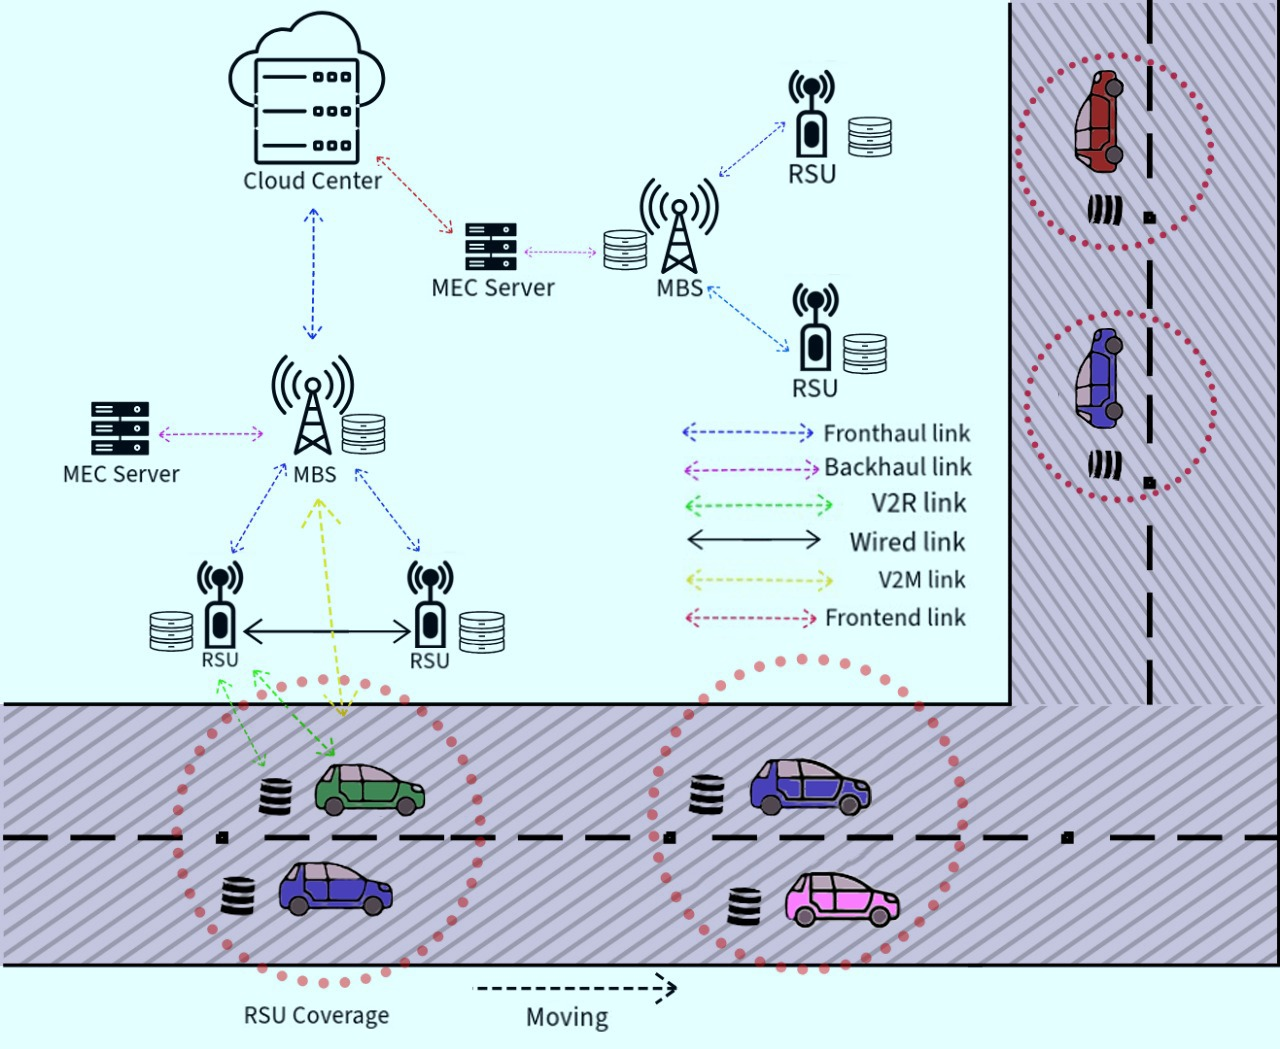
\includegraphics[scale=0.19]{images/general_vec_system_v2.png}
\caption{A generic system of vehicular edge computing integrating edge nodes (RSUs, MBSs, MEC servers) with vehicles for low-latency, high-bandwidth processing. This enables real-time data processing and decision-making, improving road safety and traffic efficiency.}
\label{fig:vec_system}
\end{figure}
Addressing communication inefficiencies in federated vehicular networks (FVN) by  \cite{r7}, the FedAGL framework incorporates adaptive parameter control, genetic algorithms, and long short-term memory (LSTM) techniques to optimize communication efficiency, thereby improving network performance. The paper  \cite{r8} proposes a three-layered VEC framework and presents a low-complexity heurstic algorithm for resource allocation, contributing to the optimization of energy consumption and resource allocation in vehicular computing systems. Yang et al. \cite{r9} discuss the significance of cooperative caching and the potential of the PBC scheme to optimize content caching and enhance user experience in VEC environments through asynchronous FL and RL techniques.
The studies \cite{r10}, \cite{r10_1} propose a collaborative caching technique that focuses on vehicular mobility patterns and further introduces a DRL content prediction framework for VEC, aiming to improve cache hit rates and mitigate latency challenges in dynamic vehicular environments. Zhang et al.  \cite{r11} presented a federated learning framework for VEC, enabling collaborative model training for tasks like traffic congestion prediction while preserving data privacy. Challenges remain due to the dynamic nature of vehicular data and constraints on in-vehicle computing resources. 

These are some survey studies discussing the basic concept and technologies about FL and the enhancement of learning efficiency, privacy and security issues.  \cite{r13}, \cite{r14}, \cite{r15} involves proposing a novel concept of Federated vehicular networks (FVN) to support data- and computation-intensive tasks in vehicular networks. The authors focuses on utilizing Federated learning within FVN and presented the architecture of FVN, highlighting the Federated vehicular cloud's (FVC) central component. The paper explores routing inside FVCs and offers first fixes as well as assessment findings. The authors hope to perform in-depth research on routing and caching algorithms, modify solutions for Blockchain-based reputation and payment support, and create a simulation framework for comparing various Federated Learning methods in FVN. 
\cite{r16} Ding et al integration of blockchain technology enhances the security of AI models in edge computing by decentralizing control, ensuring data integrity through immutable blocks, providing security against external attacks, promoting trust and transparency among participants, and reducing communication costs. Blockchain technology reduces single-point failures, improves training dependability, and enables all clients to validate and track the training by doing away with the requirement for a centralized server in federated learning training. \cite{r17} propose a novel caching scheme, termed Mobility-aware proactive edge caching (MPCF), that addresses the challenges of content delivery in dynamic vehicular networks. The scheme leverages federated learning to enable vehicles to collaboratively predict content popularity based on their mobility patterns while maintaining user privacy. By employing a Context-aware Adversarial AutoEncoder for accurate content prediction and integrating a mobility-aware cache replacement policy. 
Traditional standard solutions \cite{r20}, \cite{r21}, \cite{r21_1} in IoT and edge computing environments use data aggregation algorithms to protect data privacy. However, these methods face challenges such as poor caching performance, which results in suboptimal data transfer and processing. \par

Current research on vehicle privacy protection primarily focuses on differential privacy \cite{r22}, \cite{r23}, and deep learning methods \cite{r24}, \cite{r35}. While these approaches offer some degree of data protection in centralized machine learning training, there remains a risk of privacy leakage from the data uploaded by vehicles. These techniques are only able to partially hide the centralized training data security vulnerabilities. FL is regarded as the best option since it preserves training quality and offers improved vehicle data security. In FL, privacy is adequately protected because each car conducts individual model training rather than transferring actual data to a central server. This decentralized learning strategy protects privacy while guaranteeing the integrity of the data and providing a superior joint model. \cite{r26} paper proposed a novel proactive content caching method called Federated learning-based proactive content caching (FPCC), which utilizes a collaborative stacked autoencoder and federated learning to predict the future popularity of content while ensuring user privacy. By allowing users to independently compute updates to a shared global model based on their local data, the FPCC scheme aims to enhance cache efficiency and reduce user latency in edge computing environments, particularly in the context of increasing mobile data traffic and the demand for video streaming services. \cite{r27} paper explores the integration of Transformers and federated learning to enable privacy-preserving cooperation among autonomous vehicles. By leveraging the unified representation capabilities of Transformers for multi-modal data and the distributed learning framework of federated learning, it proposes a hierarchical structure that includes Vehicular Transformers, Federated Vehicular Transformers, and their Federations. Mahmood et al. \cite{r28} introduce RICH (RoadsIde Cache), an innovative edge caching scheme for 5G networks designed for connected cars. RICH optimally caches content at edge nodes based on vehicle mobility patterns to ensure in-order delivery of content chunks. It employs probabilistic caching that utilizes user trajectory data and dwell time estimates, improving cache hit rates and minimizing backhaul traffic. Cheng et al. 
% \cite{r29} introduces the IoV Backbone Net (IoVB-net), a structure that uses backbone nodes for efficient message forwarding, even in challenging scenarios. It also proposes an accessibility model and a routing method based on this model, which improves packet delivery rates and reduces latency compared to traditional routing methods. Ndikumana et al. 
\cite{r30} proposes a caching solution for self-driving cars using deep learning to predict content caching based on passengers' features, with caching decisions supported by nearby Multi-access edge computing (MEC) servers. It includes models for communication, caching, and content computation to optimize retrieval and storage while minimizing downloading delays. 

The literature clearly indicates that vehicle motion significantly impacts communication latency, but this is not the sole concern. Furthermore, no research has yet developed a cooperative caching system in VEC that considers both vehicle mobility and vehicle user privacy.\par


\section{Preliminary}

\subsection{FL Definition}
FL is a unique machine learning paradigm in which the model training process is decentralized over several edge devices, such as servers, smartphones, and Internet of Things devices, rather than aggregating data into a single place. In industries like healthcare or finance where data security and privacy are top priorities, a decentralized approach is especially beneficial.

Let us have a server and $N$ clients participating in an FL training process to learn a global model $w^t$. assume $w^t_j$ is of client $k$ at time $t$ having $D_j = \{\mathcal{X}_j, \mathcal{Y}_j\}$ private dataset points, where $\mathcal{X}_j$ and $\mathcal{Y}_j$ denote the data feature set and their true label set respectively. Then federated stochastic gradient descent (FedSGD) enforces all clients to form a full (non-stochastic) batch to compute gradient decent ($f$) in each iteration as follows (at the client):   
\begin{equation}
\label{fl_weighted_update_gd}
\Delta w^{t+1}_j = w^{t}_j - f(w^{t}, D_j); \;\;\; \forall{j} \in [1,N] 
\end{equation}
or,
\begin{equation}
\label{fl_weighted_update_gd2}
\Delta w^{t+1}_j = w^{t}_j - \eta \nabla \sum_{(x,y)\in D_j} \frac{1}{|D_j|} \mathcal{L}(f_w(x),y,w) 
\end{equation}
where $\eta$ learning rate and $\mathcal{L}(f_w(x),y,w)$ is the loss of data point $(x,y)$ with weight parameter $w$. Assume $|D|=\sum_{j=1}^{N} |D_j|$ compute the total number of data points from all the clients.  At the server, FedSGD aggregation step is expressed as: 
\begin{equation}
\label{fl_server_aggregation}
w^{t+1} = w^{t} + \sum_{j=1}^{N} \dfrac{|D_j|}{|D|} \Delta w^{t+1}_j 
\end{equation}
FedAvg where the server eventually computes the weighted average in FL after receiving the gradient descent of the current model using private data at each client. Each participant tends to optimize
the model $w^t$ by running various epochs utilizing optimizer SGD that uses mini-batches prepared from the private/local dataset points $D_j$. The resultant updated weight vector is described as follows:
\begin{equation}
\label{fl_weighted_update_sgd}
\Delta w_j^{t+1} = w_j^{t}  - f_{SGD}(w^{t}, D_j), \;\;\; \forall{j} \in [1,N]
\end{equation}
\begin{equation}
\label{fl_weighted_update_gd2}
\Delta w^{t+1}_j = w^{t}_j - \eta \sum_{(x,y)\in D_j} \dfrac{|D_j|}{|D|}  \nabla \mathcal{L}(f_w(x),y,w)
\end{equation}
Eventually, all participants compute their weight-updates $\Delta w^{t+1}_j$ and upload to the server, where weighted averaging is used to aggregate their data samples according to the Eq. \ref{fl_weighted_update_gd}. The server optimizes the global model using FedAvg.
Since the FL framework spreads the processing throughout the edge nodes, it helps to maintain the privacy of edge data and to reduce communication costs by sharing the lightweight hyperparameters with the server. FL builds a single global model to train and predict all samples from the participating nodes. Theoretically, all data have an underlying distribution that generates the data. 



\subsection{VFL Definition}
In Vertical Federated Learning (VFL), participants are of three types: a) \textit{ Active participant}: An active organization is interested to train a VFL model and is label owner. provide data with a given sample set. Let $\{I_j\}_{j=0}^K$ be the identity space then $\{y_j\}_{j=0}^K$ be their corresponding labels set provided. b) \textit{Passive participant:} A passive organization is invited to participate in VFL training by data features it has for the same identity space $\{I_j\}_{j=0}^K$. Typically it has no labels. It provides a feature set that is exclusive and non-overlapping from that of an active participant. There can be multiple passive participants in a VFL setup. Each participant may contribute with a distinct feature set and is free to build his own model structure. c) \textit{Coordinator}: The coordinator acts as a facilitator in the VFL framework, managing communication between participants and orchestrating the collaborative model training process. This role involves ensuring the secure exchange of intermediate data, such as gradients and embeddings, while safeguarding the privacy of individual participants' data. The coordinator may be an active participant or a trusted third party with expertise in secure communication protocols.

\subsection{Why HFL over VFL}
Hierarchical Federated Learning (HFL) is superior to VFL for distributed systems due to its scalability, efficiency, and adaptability. Unlike VFL, where all clients communicate directly with a central server, HFL uses a hierarchical structure that aggregates local updates at intermediate nodes (e.g., edge servers) before reaching the central server. This reduces communication overhead, enhances privacy by limiting direct exposure of data, and ensures faster local decision-making, which is crucial for latency-sensitive applications like vehicular networks. HFL also excels in handling heterogeneous clients with varying resources and data distributions, making it highly adaptable and robust. In distributed cache optimization, HFL minimizes network strain, reduces latency, and balances computational loads, making it the ideal choice for real-time, decentralized systems like vehicular networks.

%  \subsection{VFL categories}    

% \\ \\
% \textit{Heterogeneous vertical federated learning}: In this category, participants possess diverse data distributions, which can pose challenges for model convergence. Variations in data characteristics, such as scale, distribution, or feature types, necessitate careful preprocessing techniques, including normalization and feature selection, to harmonize the datasets. Examples of heterogeneous VFL scenarios include collaborations between entities from disparate domains, such as healthcare and finance.
% \\ \\
% \textit{Homogeneous vertical federated learning}: Here, participants exhibit similar data distributions, simplifying the model training process. Participants from comparable domains, such as different branches of healthcare or retail, contribute data that is more aligned in terms of scale, distribution, and feature types. As a result, preprocessing requirements are reduced, and model convergence may be more straightforward compared to heterogeneous VFL scenarios

\section{Methodology}

\subsection*{Problem Formulation}
\begin{figure*}[t]
\centering
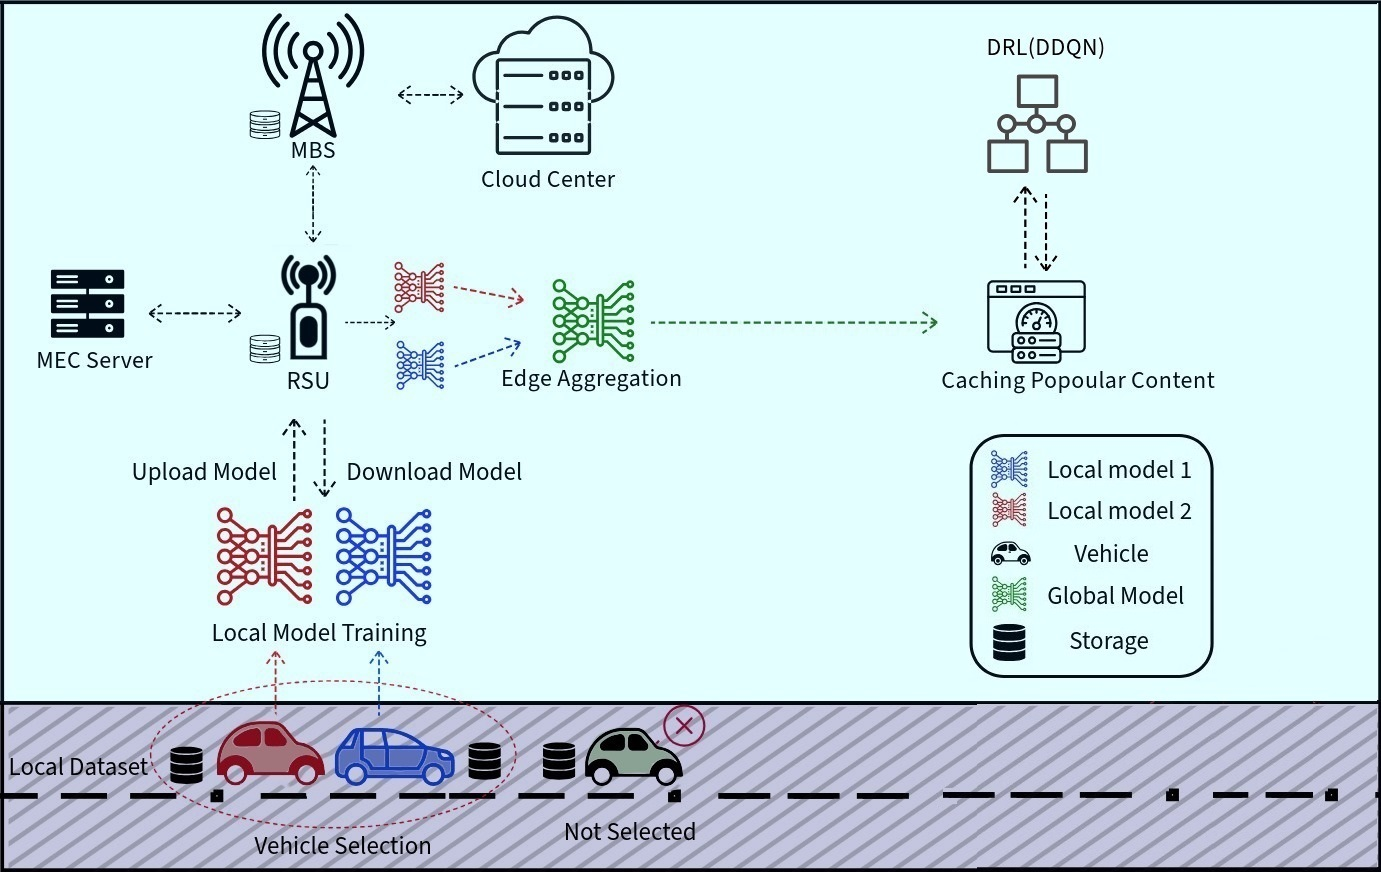
\includegraphics[scale=0.47]{images/proposed_probability_based_caching_fx_v3.jpg}
 \caption{Proposed Popularity Based Caching Framework utilizing the global model
parameters to predict content popularity and make intelligent
caching decisions at MBSs and MEC servers. }
\label{fig:PBC}
\end{figure*}
Think of \( V \) as the collection of all moving cars inside a network of roads. Our goal is to choose \( M \subseteq V \), a subset of vehicles, to take part in a training task. The cars in \( M \) are serviced by a nearby RSU, which covers an area \( \Phi \). Any vehicle's moving speed is represented by \( v_i \), while the distance traveled within this coverage region is denoted by \( d_i \). The duration that a car remains in the coverage region, \( T_{s,i} \), may be computed as follows:

\begin{equation}
T_{s,i} = \frac{\Phi - d_i}{v_i}
\end{equation}

Our objective is to enhance the coverage area's vehicle selection mechanism in order to enable more automobiles to successfully complete the training process and raise the global model's accuracy as shown in Fig. \ref{fig:PBC}. We choose the vehicle such that it resides in the RSU cover area for the travel time more than the average of the combined training time (\( T_{\text{train}} \)) and inference time (\( T_{\text{inf}} \)). This can be stated mathematically as:
\begin{equation} \label{eq:7}
T_{s,i} > T_{\text{train}} + T_{\text{inf}}
\end{equation}
With an emphasis on the parts and their interactions, the Vehicular Edge Computing (VEC) system is designed to take advantage of collaborative caching and asynchronous federated learning. Three levels are involved in how the VEC system functions in an urban setting: \textit{High Layer:} The cloud provides vast computational and storage capabilities and links to worldwide cloud services. \textit{Mid Layer:} Edge computing and services are provided by MEC servers and MBS, which are installed at the edge of the MBS coverage region. \textit{Low Layer:} The vehicle layer made up of moving cars and RSUs inside their respective coverage zones.


The vehicular network is envisioned by the PBC scheme as a data storage system, in which every car serves as a data storage node. These cars retain comprehensive vector-based history data on VUs, such as contact details, content requests, and related ratings.
Each vehicle divides its data into two parts: training set and testing set at random in order to make the most use of this data. While the testing set evaluates the model's performance and enables ongoing modification and adaptation, the training data is used for initiating learning mechanism. Vehicle time in MBS coverage region is broken down into many rounds. Vehicles choose data at random from their testing sets for each round, then they request access to the content from RSUs.
While each RSU has limited storage and can only hold a fraction of the data, the MBS acts as the central storage node and has adequate capacity to cache all accessible content. Based on various parameters, vehicles can retrieve data from nearby RSUs, the MBS, or local RSUs. This increases system responsiveness and efficiency and allows for more agility to meet VU needs.

The system uses a ranking system to determine VU interest in data. A rating of 0 denotes neither disfavor nor lack of requests, although higher ratings reflect increased interest. Using this input, data distribution tactics can be optimized and more personalized services can be offered. It is necessary to go into further depth on the key ideas showed in Fig. \ref{fig:PBC}  before going into the framework itself.

\textbf{a) Roadside Unit (RSU):} This unit holds content that is regularly requested and provides it to cars as needed. The local RSU responds to the vehicle's request immediately if it has the desired content in its cache. If not, a nearby RSU receives the request and handles it further.

\textbf{b) Neighboring RSU:} This unit is located at the periphery of the road network, just like the local RSU, except it might be farther away from the car yet still be reachable by radio. When the local RSU forwards requests to it, it looks through its cache to see if the required data is there. It transmits the data straight to the car if it is accessible and connectivity with the vehicle is reliable. If not, it returns the request for delivery to the nearby RSU.

\textbf{c) Macro Base Station (MBS):} To enable vehicle data uploads and downloads, the MBS offers high-speed data connection. The vehicle sends a request to the MBS if the required data is not cached by either the local RSU or the nearby RSUs. After that, the MBS gets the required content and sends it straight to the car.

\textbf{d) Mobile Edge Computing (MEC) Server:} Situated close to the MBS, this edge layer component has a sizable amount of processing and storage capacity. Through communication with the MBS, edge computing services provide instructions to it. The server manages local edge computing jobs, providing RSUs and automobiles with high-performance, low-latency services. A sophisticated and effective communication system incorporating several MBSs, RSUs, MEC servers, cloud servers, and automobiles is constructed in this urban vehicular network scenario. The city's ability to have consistent vehicle connection depends on the MBS and RSU locations. Key edge sites within the urban environment are where MBSs are deployed. Within the coverage area of each MBS, a series of evenly spaced RSUs is organized. Furthermore, a highly integrated network may be formed by MBSs interacting with MEC servers and MEC servers interacting with the cloud server.
Under this approach, automobiles are represented by the set:
\begin{equation}
\mathcal{X} = \{ X_1, X_2, X_3, \ldots, X_n \}
\end{equation}
where the variable \( n \) represents connected vehicles' count. The data transfer among neighboring RSUs is accomplished through physical wired links. Within a given round, every vehicle follows the same communication protocol; however, in subsequent rounds, vehicles might need to modify their communication plans to accommodate evolving demands or environmental circumstances.


The Macro Base Station (MBS) establishes a robust backhaul link to the MEC server and connects through a fronthaul link to the cloud server. Furthermore, it's a frontend link that connects the MEC and cloud servers. To support caching, the infrastructures of MBSs and RSU servers are equipped with edge computers. RSUs primarily store frequently requested content by nearby vehicles, which facilitates quicker data access while the vehicles are in motion. By controlling and distributing the cached content directory to linked RSUs, the MBS enhances reaction times and data transfer rates. Every RSU offers assistance to its related vehicles even as they move across different MBS coverage areas. This seamless handover ensures continuous connectivity for vehicles throughout the city, offering reliable and efficient communication services to both vehicles and drivers. The speeds of vehicles are regarded as random variables that are independent with identical distributions. The following represents the range of vehicle speeds:
\begin{equation}
\mathcal{S} = \{ S_1, S_2, S_3, \ldots, S_p \}
\end{equation}
where each \( S_i \) denotes a vehicle's velocity. These speeds are modeled using truncated Gaussian distributions \cite{r30a}, which restrict them to a specific range. This approach better reflects real-world vehicle dynamics, keeping in mind the different road situations and traffic laws that impact velocity.
During each experimental round, vehicles maintain a constant, specified speed, ensuring stable and controlled experiments. This configuration makes it possible to analyze communication results and vehicle behavior in detail at different velocities. A car transmits service or data requests to a nearby RSU as it moves within its receiving area, enhancing traffic efficiency and driving experience by providing access to necessary services or data. In the \( j \)-th experimental round, The quantity of automobiles in the nearby RSU coverage region is indicated as \( \mathcal{X}_j \). The set of vehicles can be represented as:
\begin{equation}
\mathcal{X} = \{ \mathcal{X}_1, \mathcal{X}_2, \mathcal{X}_3, \ldots, \mathcal{X}_q, \ldots, \mathcal{X}_j \}
\end{equation}
The assumed set of vehicle speeds in the \( j \)-th round is:
\begin{equation}
\mathcal{U} = \{ U_1, U_2, U_3, \ldots, U_q, \ldots, U_j \}
\end{equation}
where \( U_q \) denotes the participant's car speed. The data distribution of the cars' speed is modeled using a truncated Gaussian distribution.
\begin{algorithm}
\caption{Global Model Update with Vehicle Data}
\label{alg:global_model_update}
\begin{algorithmic}[1]
\REQUIRE Global Model $\beta_{\text{global}}$ Vehicles info, including speed, direction, and training data.
% \ENSURE Modified Global Model $G_{m}$.

\STATE \textbf{Initialization:} Load arguments and initialize parameters.
\STATE Set device (GPU/CPU).
\STATE Load and prepare data for training and testing.
\STATE Initialize environment, global model, and local models.
\STATE Set global weights and tracking variables.

\FOR{each epoch $idx$}
    \STATE Print epoch details and set $\beta_{\text{global}}$ to training mode.
    \STATE Adjust local learning rate $\text{local\_lr}$ based on epoch.
    \STATE Compute V2I rate and update performance metrics.
    
    \FOR{each vehicle $V_{e_i}$}
        \STATE Calculate staying time $T_{\text{staying}, e, i}$ using Eq.(\ref{eq:7}).
        \IF{$T_{\text{staying}, e, i} > T_{\text{training}} + T_{\text{inf}}$}
            \STATE Update local model asynchronously.
            \STATE Adjust and aggregate local weights into $\beta_{\text{global}}$. Eq. (\ref{eq:9}).
            \STATE Track epoch duration.
        \ENDIF
    \ENDFOR
\ENDFOR

\IF{last epoch}
    \STATE \textbf{Testing and Evaluation:} Evaluate caching strategies (Random, Oracle, Greedy, Thompson Sampling).
    \STATE Compute cache efficiency and delays for each strategy.
\ENDIF

\STATE \textbf{Environment Update:} Update vehicle positions and speeds. Renew simulation channels and fading conditions.

\IF{maximum epochs are exceeded}
    \STATE Terminate training.
\ENDIF
\STATE \textbf{return} Updated joint global-model \beta_{\text{global}}.

\end{algorithmic}
\end{algorithm}
To maximize cache efficiency and improve access speed, popular content should be strategically placed on RSUs. Understanding content popularity is crucial as it is influenced by factors such as user demographics and vehicle mobility patterns. Our PBC approach aims to make well-informed caching decisions for RSUs by considering relevant parameters and accurately predicting content popularity. By intelligently managing caches, we can enhance network speed, user experience, and edge computing performance within vehicles. Furthermore, the integration of cache management with content popularity prediction enables smooth content distribution and enhances the performance of the vehicular edge computing environment.

However, city traffic environments pose challenges due to high vehicle mobility and volume. When vehicles request content from their current RSU and it is not cached, they must retrieve it from nearby RSUs or the MBS. Moreover, the limited coverage area of RSUs restrict the time available for content downloads. To mitigate these problems, we suggest a caching strategy Fig. \ref{fig:PBC}. Utilizing vehicle mobility data, including position and speed, facilitates the selection of appropriate cars for caching and model training. Vehicles upload updated models to their local RSUs after local training, and these RSUs then update the global model. The global model parameters are used by the edge layer to predict content popularity and make informed caching decisions at MEC servers and MBSs.

\subsection{The Proposed Asynchronous FL Algorithm} 


\textbf{\textit{1) Vehicle Selection:}} In advancing innovation in telematics, the strategy for selecting vehicles plays a crucial role. The limited coverage of RSUs presents a challenge in situations where highly mobile vehicles can find it difficult to complete Federated Learning training in the allotted time, potentially resulting in degraded performance of the global model and cache performance. To improve the accuracy of global models, aggregating the best car model updates is crucial at RSU server. We aim to identify the vehicles which remain within the coverage area of a local RSU for sufficient time to guarantee their complete participation in  FL training and the successful completion of the model training process.

Initially, the vehicle selection process starts where each vehicle transmits its mobility characteristics, including its closest RSU, displacement from the RSU, speed and the distance traveled within the RSU's cover area. The time interval that each car resides in the RSU's cover area is determined by the local RSU through the use of these features in the formulation of an advanced vehicle selection logic. On the basis of these parameters, vehicles are then chosen for training. The duration that a car $V_i$ stays in the local RSU cover area is determined as follows:
\begin{equation}
T_{\text{stay}, i} = \frac{D - d_i}{v_i},
\end{equation}
where $v_i$ is the vehicle's speed, $d_i$ indicates the vehicle's travel distance inside the area of coverage of the local RSU's, and $D$ stands for the coverage area. A vehicle must remain in the coverage area for a sufficient period in order to guarantee that the training process is successful and yields successful and effective outcomes.

Consequently, it is important to ensure that a car remains inside the RSU area of coverage for an extended amount of time than the average for both the inference time ($T_{\text{inf}}$) and the training time ($T_{\text{train}}$). The constraint that must be satisfied for the vehicle to be chosen for the asynchronous FL-based learning process else it will be ignored. This approach aims to enhance both the sustainability and performance of the entire connected vehicle network while further optimizing the joint global model.




\textbf{\textit{2) Model Download:}} The objective of this stage is to develop a joint global model which is utilized at local RSUs. An Variational Autoencoder (VAE) is first used to establish RSU during the first round, laying the groundwork for the global model $\beta_{\text{global}}$. This model serves as a foundational element for forecasts of popular content in the future. RSU methodically updates the global model $\beta_{\text{global}}$ in each following cycle so that it is in line with the most current vehicle data. This iterative procedure emphasizes how crucial ongoing modification is to preserving the precision and dependability of the model.

After that, the distribution of the model becomes the main priority. The RSU meticulously refines the revised global model $\beta_{\text{global}}$, which is subsequently sent to a subset of cars. With the help of this intelligent model, cars may conduct thorough training and research thanks to its advanced learning platform.


\textbf{\textit{3) Model Training:}} In a distributed machine learning setting, it is essential to use iterative implementation and local model updates to provide cooperative learning across a fleet of automobiles. With this method, every chosen car iterates $z$ times to improve its local model, which aids in the global model's optimization. At each of these phases, gathering data is essential.
A chosen vehicle $V_i$ updates its local model at each iteration $r$, and a random sample of data $d^r_i$ is taken from the entire training set. The utilization of a random sampling approach is crucial in preserving data variety.
Two crucial phases are involved in local model updates to capture the inherent qualities of the data: hidden feature extraction and data reconstruction. The training data is sent into an Variational autoencoder during the data reconstruction process, enabling it to use its hidden layer characteristics to identify the fundamental patterns within the original data. $x$. The Variational autoencoder reconstruction of the data, $x'$, preserves the essential elements of the original data.

\textbf{\textit{4) Model Upload:}} Every car communicates its updated local model to the nearby RSU for aggregation into a global model following the completion of local training. The main goal is to secure the privacy of personal data while collaboratively optimizing the global model.

\textbf{\textit{5) Aggregation:}} The car $V_i$ sends its updated parameters $\beta_i$ to the local RSU once its local model update is complete. Next, the global model parameters are adjusted by the RSU  based on how the performance of the global model is affected by the various residency durations of the cars. The following method is used to make the adjustment:

\begin{equation} \label{eq:9}
\beta_{\text{global}} = \beta_{\text{global, prev}} + \eta \sum_{i=1}^{N} (R_i \cdot \gamma_i \cdot \beta_i),
\end{equation}
where the step size for the model parameter update is determined by the parameter $\eta$. The coefficient $R_i = \frac{d_i^l}{d_i^a}$ shows the proportion of the overall data size ($d_i^a$) of the chosen vehicle to the local data size ($d_i^l$). The value of $\gamma_i$ is calculated as follows:

\begin{equation}
\gamma_i = \alpha_1 (C - d_i) + \alpha_2 \left( \frac{s}{T_{e, i}} \right),
\end{equation}

where $s$ indicates each item's size, $\alpha_1$ denotes the weight for distance traveled, $\alpha_2$ is the weight coefficient for controlling the transmission delay. It's observed that $\alpha_1 + \alpha_2 = 1$. Normalization is carried out in order to preserve stability and control while modifying the trade-off variables and to stop any weight modification from creating instability in the overall results:

\begin{equation}
\gamma_i = \alpha_1 \log\left( \frac{C}{d_i} \right) + \alpha_2 \log\left( \frac{T_{e, i}}{T_{\text{max}, e}} \right),
\end{equation}
where the maximum transmission rates, $T_{\text{max}, e}$, among all the cars in the local RSU's coverage region are used to do this normalization. The RSU distributes the modified global model to every vehicle at the start of the subsequent iterative optimization cycle. The RSU continues to refine the global model after the allotted number of iterations has been achieved in order to generate a more efficient version of $\beta_{\text{global}}$. The intricate process of forecasting popular material is described in depth in the next section.

\begin{algorithm} [t]
\caption{Recommendation System Algorithm with Popularity-based Caching}
\label{alg:recommendation_system}
\begin{algorithmic}[1]
\REQUIRE User-movie matrix $U$; Test dataset $T$; Model weights $W$; Cache size $C$; Probability $e$; Maximum movie ID $M$
\ENSURE Recommended movies list

\STATE Compute user-movie compressed matrix $U_{\text{cos}}$ from $U \& W$
\FOR{each user $u$ in $T$}
    \STATE Calculate similarity of $u$ to all users: \\$S[u] \leftarrow \text{cosine\_similarity}(U_{\text{cos}}, U_{\text{cos}}[u])$
    \STATE Sort users by similarity and select top 10 similar users: \\$S[u] \leftarrow \text{top\_k\_similar\_users}(S[u], 10)$
    \STATE Aggregate watch history from similar users: \\$H[u] \leftarrow \text{aggregate\_history}(S[u], T)$
    \STATE Compute recommendations for $u$: \\$R[u] \leftarrow \text{top\_items}(H[u], C)$
\ENDFOR

\STATE \textbf{Popularity-based Caching:} 
\STATE Compute movie popularity from \\$T$: $P[m] \leftarrow \text{count\_movie\_occurrences}(T, m)$
\STATE Recommend top $C$ most popular movies:\\ $R_{\text{pop}} \leftarrow \text{top\_items\_by\_popularity}(P, C)$

\end{algorithmic}
\end{algorithm}
\subsection{ Content Popularity Algorithm}

\textbf{\textit{1) Data preparation and Matrix construction:}} The recommendation system begins with data sampling and preprocessing. At each participant client or user group, local data is split into a training set and a test set. For each client, a user-item matrix (such as user-movie-rating or vehicle-user-content matrix) is constructed, where rows represent users (or Vehicle Users, VUs) and columns represent items (movies or content). Alongside the interaction data, additional user attributes (e.g., gender, age, occupation for movies, or personal information for VUs) are incorporated into the matrix. To address the common issue of sparse data in these matrices, where many entries might be zero due to a lack of interaction, we employ a Variational Autoencoder (VAE). This model effectively handles sparse data by learning to reconstruct missing values in a way that captures the underlying distribution of the data. By training the VAE on our dataset, we generate a reconstructed matrix that minimizes zeros, providing a more accurate reflection of user or VU preferences. This refined matrix serves as a robust basis for further analysis.

\textbf{\textit{2) User Clustering Using Cosine Similarity:}} After refining the user-item matrix, the next step is to identify similar users, or "neighbors," for each target user in the test dataset. This is achieved using the Cosine Similarity metric, which measures the similarity between vectors in a multi-dimensional space. For a target user or VU, the cosine similarity between their vector and those of all other users is computed. The similarity score is defined as:

\begin{equation}
\text{simi}(x, y) = \frac{C_i(x,:) \cdot C_i(y,:)}{\|C_i(x,:)\|_2 \times \|C_i(y,:)\|_2}
\end{equation}
where \( C_i(x,:) \) and \( C_i(y,:) \) are row vectors representing user or VU features. This metric yields a value between -1 and 1, where a higher value indicates greater similarity in preferences. Based on these similarity scores, the system selects the top 10 most similar users for each target user, forming a cluster that helps predict the target user's preferences more accurately.

\textbf{\textit{3) Generating Recommendations Using Collaborative Filtering:}} With the clusters of similar users identified, the system proceeds to generate recommendations. This involves aggregating the viewing or interaction history of the similar users. For movie recommendations, the system compiles a list of movies watched by these users, counts the frequency of each movie, and selects the top-N most-watched movies as personalized recommendations for the target user. This approach ensures that the recommendations align closely with the user’s preferences.

\textbf{\textit{4) Content Popularity Algorithm for Vehicle Users:}} For vehicle users, after clustering based on similarity, the system focuses on predicting popular content among the VUs. The ratings of the similar VUs on different content are aggregated to form a new rating matrix. The content items are ranked based on their frequency of non-zero ratings among these neighbors. The top-K most popular content items are then selected and uploaded to the local RSU. The RSU further filters and selects the most popular content to ensure that the most relevant and in-demand content is readily available to vehicle users.

\begin{algorithm}[t]
\caption{Double Dueling Deep Q-Network (DDQN) Algorithm}
\label{alg:dueling_dqn}
\begin{algorithmic}[1]
\REQUIRE Total episodes $Ts$, replay buff. $D$, min-batch size $I$
\ENSURE Optimal caching policy

\STATE Set up the targeted network with parameters $\theta'$ and the prediction network with initial parameters $\theta$.

\STATE Set up initially replay buffer $D$ as empty

\FOR{each episode $r = 1$ to $Ts$}
    \STATE At local RSU, choose $c \in F_c$ popular content items.
    \STATE Choose $c$ distinct items at random from the same set for the nearby RSU.
    \FOR{each time slot $t = 1$ to $Ns$}
        \STATE Observe state $s^{(t)}$
        \STATE Compute Q-values for each action $a \in \{0, 1\}$
        \STATE $V(s^{(t)}; \theta) \leftarrow   \text{Feature Layer}$    Eq. (\ref{eq:14}).
        \STATE $A(s^{(t)}, a; \theta) \leftarrow \text{Advantage Layer}$   Eq. (\ref{eq:14}).
        \STATE $Q(s^{(t)},a;\theta) \leftarrow V(s^{(t)};\theta)+(A(s^{(t)},a;\theta)-\text{E}[A(s^{(t)},a;\theta)])$
        \STATE Choose action $a(t)$ using the $\epsilon$-greedy strategy
        \STATE Execute action $a(t)$, observe reward $r(t)$ and next state $s(t+1)$
        \STATE Cache contents not in $s(t+1)$ by nearby RSU
        \STATE Store transition $(s^{(t)}, a(t), r(t), s(t+1))$ in $D$  Eq. (\ref{eq:15}).
        \IF{size of $D$ exceeds $I$}
            \STATE Sample a mini-batch of $I$ experiences from $D$
            \FOR{each experience $(s_i, a_i, r_i, s_i')$ in the mini-batch}
                \STATE Compute target Q-value: $y_i \leftarrow r_i + \gamma \cdot \text{max}_{a'} Q(s_i', a'; \theta')$
                \STATE Update prediction network by minimizing: $(Q(s_i, a_i; \theta) - y_i)^2$
            \ENDFOR
        \ENDIF
    \ENDFOR
\ENDFOR

\end{algorithmic}
\end{algorithm}


\subsection{DRL Framework (DDQN)}
\textbf{\textit{Double Dueling Deep Q-Network (DDQN) Algorithm:}}
When dealing with situations where certain actions have little to no impact on later stages, the DDQN algorithm works well. This is owing to the fact that the DDQN method splits the Q-value into the action-dependent action advantage function (A) and the state value function (V), which both depend on the action. To tackle this specific issue, we employ the DDQN algorithm, which is more adept at managing scenarios in which not every action has a substantial influence on future states. The DDQN consists of three fundamental parts: a prediction network, a target network, and a replay buffer. While the prediction network predicts the current state-action value (Q-value) function, the target network approximates the ideal Q-value function. The feature, state-value, and advantage layers are the three layers that constitute the structure of both networks. In the replay buffer $D$, the transitions that occur in each time slot are recorded.
The algorithmic workflow of DDQN is: 

\textbf{1) Initialization:}
The prediction network parameters $\theta$ and the target network parameters $\theta'$. are initialized randomly. The contents that are requested by every vehicle in the nearby RSU (Roadside Unit) are then taken into account as input for each round $r$. 

\textbf{2) Episodes Execution:} $T_s$ episodes are processed by the algorithm. At the beginning of each episode, the local RSU randomly selects $c$ contents from the $F_c$ popular contents, while the neighboring RSU selects $c$ different contents from the same set that aren't stored in the nearby RSU. The program then repeats this process for time periods between 1 and $N_s$. 

\textbf{3) Prediction Network Operations:} The local RSU monitors the state $s^{(t)}$ at each slot $t$ and feeds it into the prediction network. For every conceivable action $a \in \{0,1\}$, The state value function $V(s^{(t)};\theta)$ and the action advantage function $A(s^{(t)},a;\theta)$ are the results of the network processing this input through the feature layer, state-value layer and advantage layer in that sequence. Next, the Q-value function is computed as follows for each action a:

\begin{equation} \label{eq:14}
Q(s^{(t)},a;\theta) = V(s^{(t)};\theta) + \left( A(s^{(t)},a;\theta) - \mathbb{Avg}[A(s^{(t)},a;\theta)] \right)
\end{equation}

In this case, the average action advantage value $\mathbb{Avg}[A(s^{(t)},a;\theta)]$ is subtracted from the Q-value computation in order to remove excessive degrees of freedom and improve algorithm stability. 

\textbf{4) Action Selection and Reward Calculation:} A technique known as $\epsilon$-greedy is used to select the action $a(t)$. This strategy helps strike a balance between trying out novel actions and sticking with the most well-known action. To put it simply, this technique selects the action for the current state $s^{(t)}$ that yields the highest Q-value. The action $a(1)$ is set to 1 at the start (slot 1). Following the selection of an action, the system advances from the current state $s^{(t)}$ to the subsequent state $s(t+1)$. The local RSU uses certain formulae to compute a reward $r(t)$. This new state $s(t+1)$ is then seen by the local RSU. In the meantime, certain popular contents not already in $s(t+1)$ are randomly selected and cached by the nearby RSU; this process is called $s_n(t+1)$. In a replay buffer $D$, the complete process, from $s^{(t)}$ to $s(t+1)$, is kept as a tuple
\begin{equation} \label{eq:15}
(s^{(t)}, a(t), r(t), s(t+1)). 
\end{equation}
\textbf{5) Replay Buffer and Mini-Batch Sampling:} The local RSU randomly picks $I$ of the recorded experiences (tuples) in the replay buffer $D$ to construct a mini-batch when the number of stored experiences exceeds a predetermined value $I$. Then, for training purposes, each experience in the mini-batch (denoted as $(s_i, a_i, r_i, s_i')$ for each $i$) is input into the prediction and target networks. 

\textbf{6) Updating the Prediction Network's Parameters:} The target network receives the current state $s_i$ for every experience in the mini-batch. The state value and the action advantage are the two outputs that the network generates after processing this input across several layers. The expected reward for every action in a given state is then determined by computing the Q-value, which is derived from these outputs. The model simplifies and stabilizes the training by computing the difference between the action advantage function and its average.
\begin{table}[t]
\caption{Cache Efficiency Values with Cache Sizes}
\label{table:cache_efficiency}
\centering
\begin{tabular}{|c|c|c|c|c|}
\hline
\textbf{Cache Size} & \textbf{PBC Eff.} & \textbf{Greedy Eff.} & \textbf{TS Eff.} & \textbf{Random Eff.} \\ \hline

50  & 14.55 & 10.45 & 6.61 & 1.32 \\ \hline
100 & 23.14 & 21.45 & 16.02 & 2.94 \\ \hline
150 & 35.55 & 29.49 & 22.26 & 5.22 \\ \hline
200 & 39.96 & 35.99 & 31.08 & 7.42 \\ \hline
250 & 45.72 & 42.34 & 36.00 & 7.94 \\ \hline
300 & 48.91 & 45.02 & 45.20 & 8.54 \\ \hline
350 & 56.23 & 50.02 & 49.23 & 8.89 \\ \hline
400 & 62.22 & 55.72 & 57.00 & 10.9\\ \hline
\end{tabular}
\end{table}
\section{SIMULATION RESULTS}
% In this part, we examined the proposed PBC scheme performance.
\subsection{ Environment Specifications}
Every car is equipped with datasets for training local models. We used the Movie Lens 1M dataset, which contains 1,000,209 ratings for 3,706 movies from 6,040 users. Each user has rated at least 20 movies on a scale from 1 to 5. The dataset also includes detailed movie information, such as geographical origin, production companies, and runtime. We use it to represent Vehicular user data with similar characteristics. We used Python 3.11 on Anaconda to simulate a vehicle-based edge computing environment in an urban setting, running on an NVIDIA RTX 3080 GPU. Visual Studio supported development and visualizations. This setup enhances realism by facilitating data sharing and cooperation among vehicles in the simulated environment.


\begin{figure}[t]
    \centering
    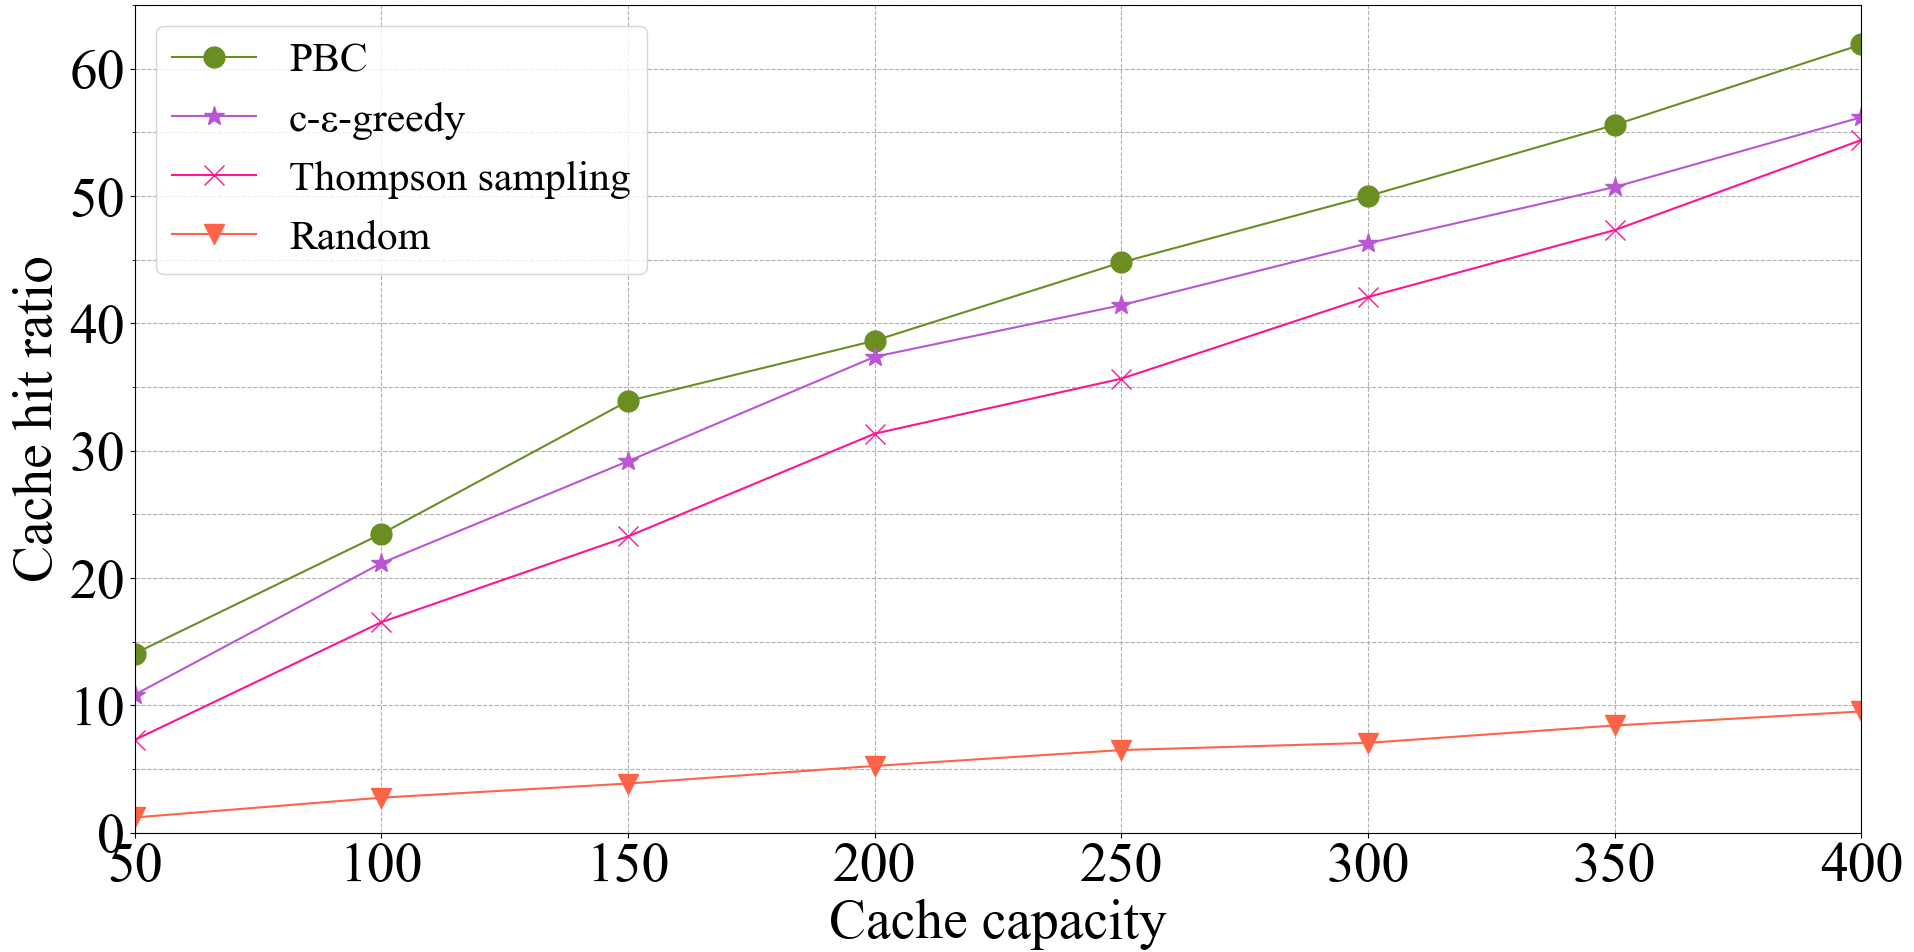
\includegraphics[scale=0.18]{images/fig 3.png}
    \caption{The graph illustrates that the PBC algorithm consistently achieves the highest cache hit rate across varying cache capacities compared to others, with all schemes showing improved hit rates as cache capacity increases.}
    \label{fig:Cache_hit_ratio}
\end{figure}

\begin{figure}[t]
    \centering
    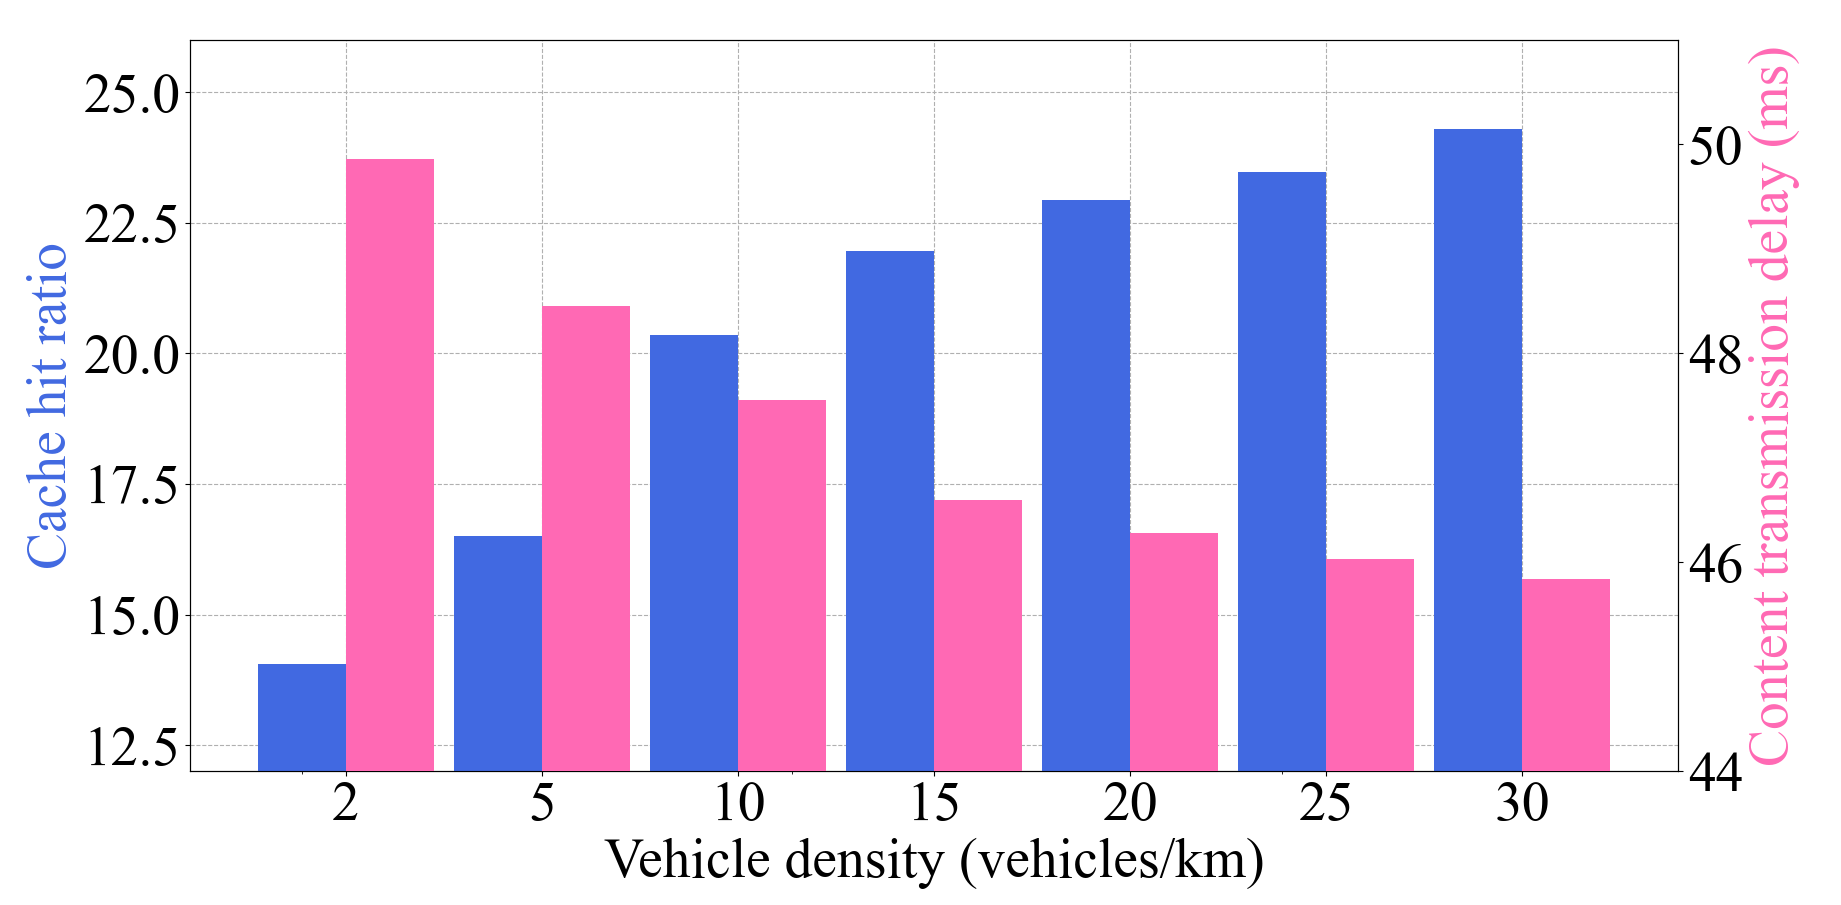
\includegraphics[scale=0.185]{images/fig 4.png}
    \caption{This graph compares vehicle density to cache hit ratio and content transmission delay. It shows cache efficiency (blue) and delay (pink) across different vehicle densities, highlighting system performance changes.}
    \label{fig:cachehitrate_correlation_with_vehicledensity}
\end{figure}

  

\subsection{ Experimental Results and  Evaluation}

The cache hit ratio and content transmission latency are the two performance indicators we use to assess the PBC method. The probability of obtaining the desired material from the nearby RSU is indicated by the cache hit ratio. A cache hit will occur if the requested material is kept in the local RSU and is accessible straight from there. It is regarded as a cache miss. We evaluate the proposed PBC algorithm against the three baseline cache techniques.


Fig. \ref{fig:Cache_hit_ratio} illustrates the average cache hit ratios of various caching strategies as a function of cache capacity. PBC performs the best, significantly increasing from 14.5\% to 62.2\% with larger cache sizes due to its effective content placement strategy. c-$\epsilon$-greedy shows moderate performance, improving from 10.4\% to 55.7\%, benefiting from a balance between exploration and exploitation. Thompson Sampling also performs well, increasing from 6.6\% to 57.0\%, with its probabilistic approach to content management. In contrast, Random Caching performs the worst, with a cache hit ratio ranging from 1.3\% to 10.9\%, as it places content arbitrarily without optimization. All strategies exhibit improved performance with larger cache sizes, highlighting that increased cache capacity enhances caching efficiency. The superior performance of PBC is attributed to its strategic approach, while Random Caching's inefficiency results from its lack of systematic content management. Fig. \ref{fig:cachehitrate_correlation_with_vehicledensity}. illustrates the effect of vehicle density on the performance of the caching system by showing two metrics: cache hit ratio and content transmission delay. The cache hit ratio, depicted by blue bars, improves as vehicle density increases from 2 to 30 vehicles per kilometer, rising from approximately 12\% to 26\%, which highlights enhanced caching efficiency with higher vehicle density. Conversely, the content transmission delay, shown by pink bars, remains relatively stable between 44 ms and 51 ms across different densities, indicating that while vehicle density significantly affects caching efficiency, it has a minimal effect on content delivery speed.

\begin{figure}[t]
    \centering
    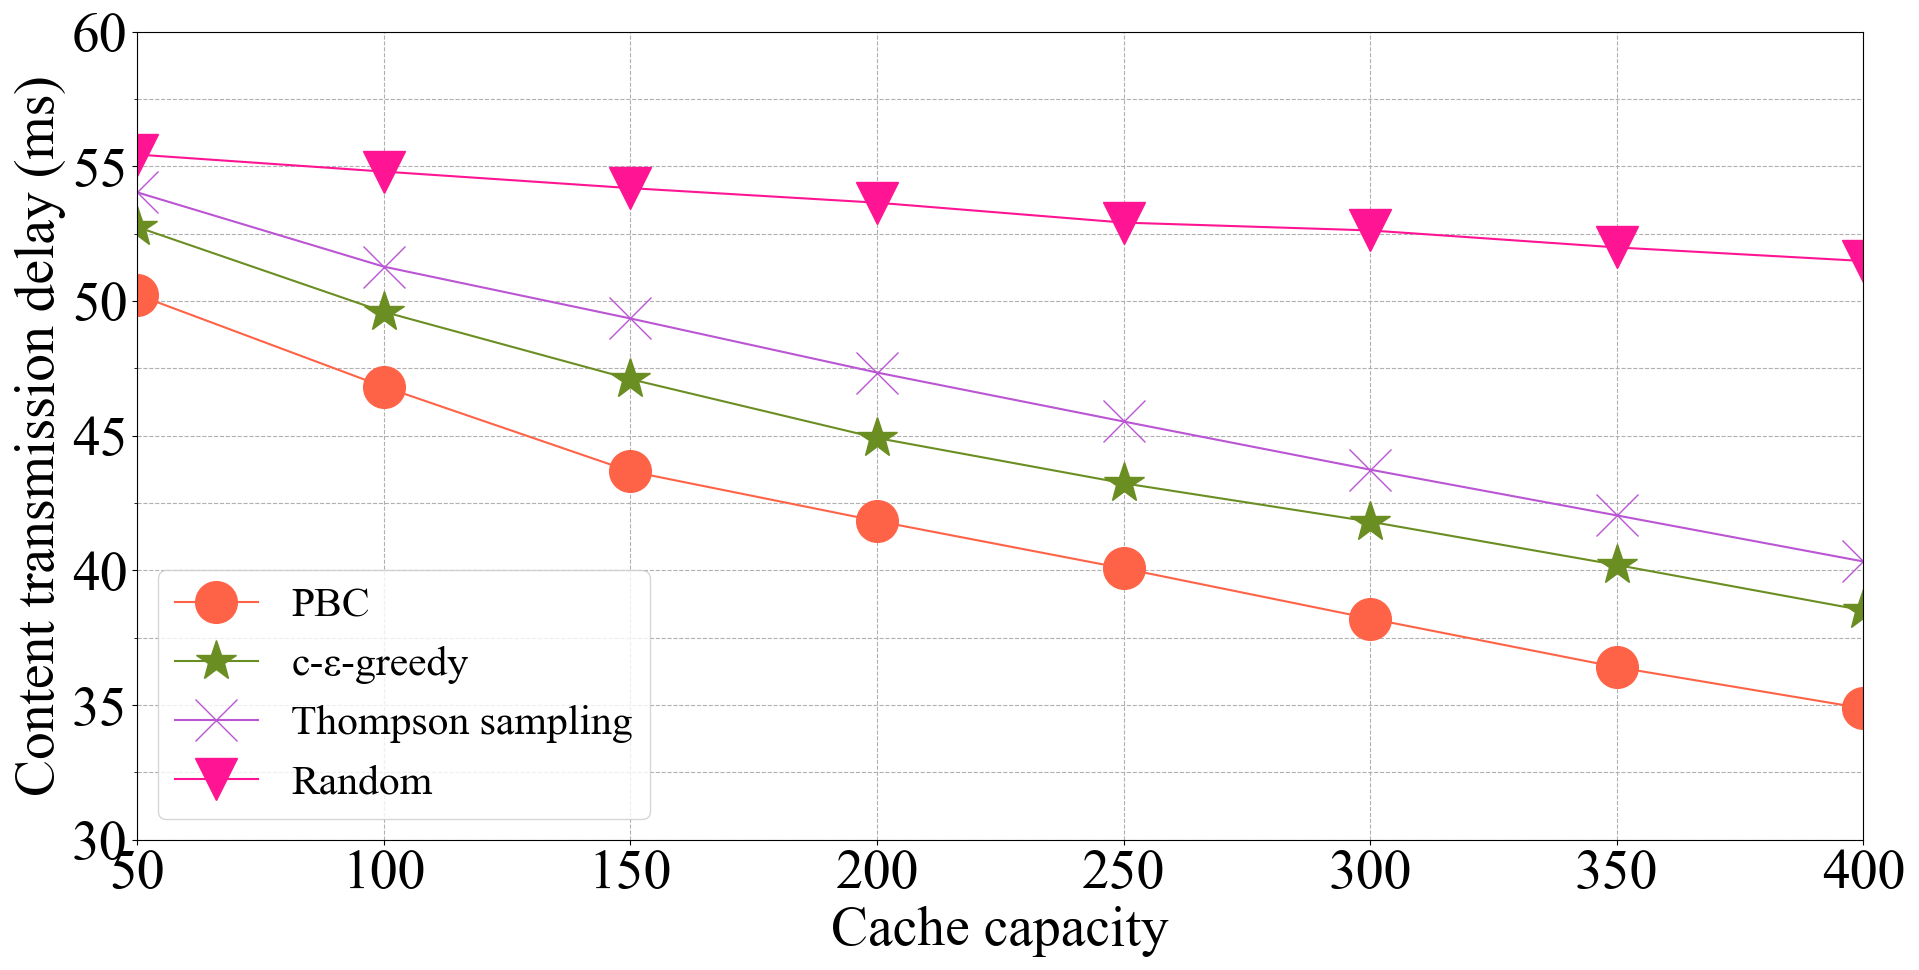
\includegraphics[scale=0.18]{images/fig 5.png}
    \caption{Content transmission delays across different caching strategies (PBC, Greedy, Thompson Sampling, and Random) as cache size varies.}
    \label{fig:cache_transmission}
\end{figure}

\begin{figure}[t]
    \centering
    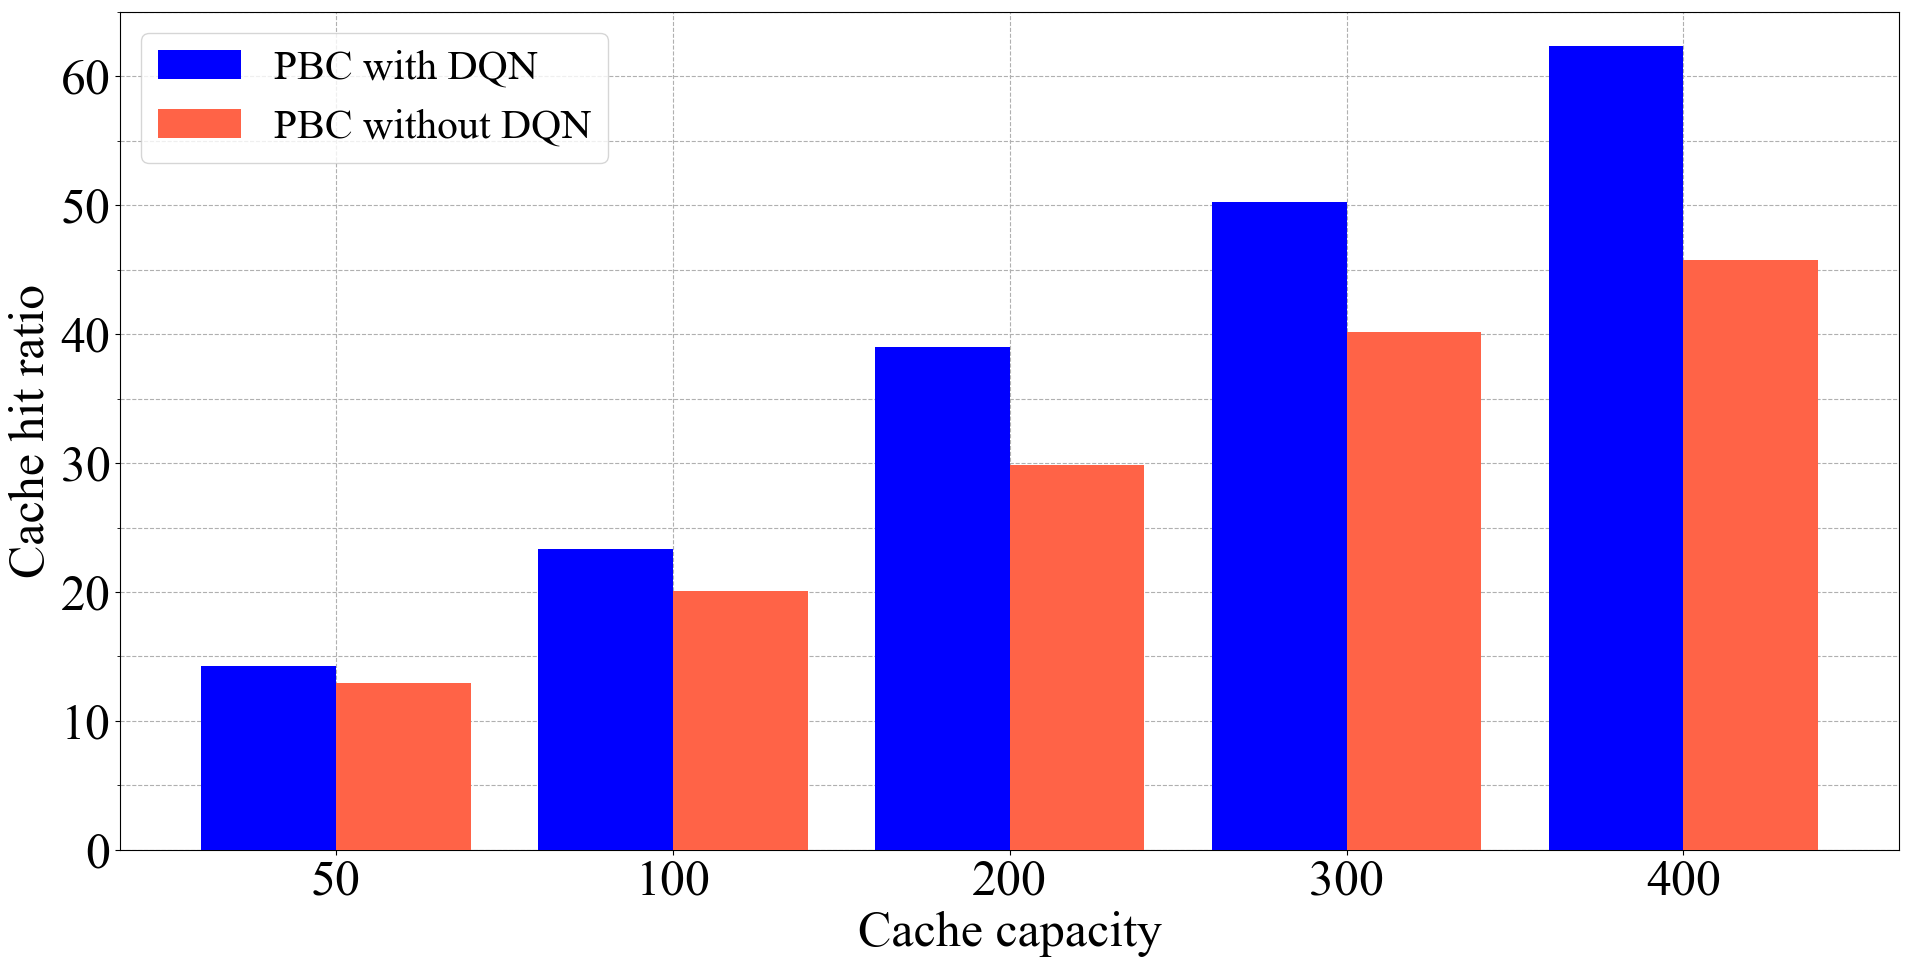
\includegraphics[scale=0.175]{images/fig 6.png}
    \caption{The PBC caching strategy with DDQN consistently achieves a higher cache hit ratio compared to PBC without DDQN across varying cache capacities}
    \label{fig:cache}
\end{figure}
Fig. \ref{fig:cache_transmission} shows that content transmission delay decreases with larger cache sizes for all strategies; PBC achieves the lowest delays. PBC excels because it prioritizes frequently accessed items, reducing cache misses and optimizing performance. Larger caches allow more data to be stored locally, enabling vehicles to quickly access data from nearby RSUs, which further reduces delays. While Thompson Sampling and c-$\epsilon$-greedy also improve with larger caches, PBC remains the most effective at minimizing transmission delays. Random caching results in the highest delays due to its lack of optimization. Fig. \ref{fig:cache} compares the cache hit ratios for PBC with and without DDQN optimization across different cache sizes. It illustrates that incorporating DDQN generally results in higher cache hit ratios compared to the standard PBC approach. For instance, at a cache size of 50, PBC with DDQN shows a hit ratio of approximately 13.77\%, while PBC without DDQN is around 12.21\%, reflecting a 1.56\% improvement. This trend continues, with the difference widening to a 17.6\% increase at a cache size of 400, where PBC with DDQN reaches a 62.2\% hit ratio compared to 44.19\% for PBC without DDQN. The graph effectively highlights that DDQN optimization leads to a noticeable enhancement in caching performance, particularly at larger cache sizes.




\subsection{CONCLUSION AND FUTURE WORK}
In this paper, we proposed a novel Popularity-based Caching scheme designed to optimize caching performance in vehicular networks. Our extensive analysis and experimental results demonstrate that the PBC algorithm consistently outperforms other benchmark caching strategies, including Greedy, Thompson Sampling, and Random Caching. The results show that PBC achieves the highest cache hit ratios across all cache sizes, with an improvement from 14.5\% at a cache size of 50 to 62.2\% at 400, significantly surpassing the next best method, Greedy, which reaches 55.7\% at its peak. Additionally, PBC demonstrates the lowest content transmission delays compared to other schemes, making it the most efficient in reducing cache misses and improving data access speed. In conclusion, our PBC scheme, especially when enhanced by DDQN, not only achieves the highest cache hit ratios but also minimizes transmission delays, making it the most effective strategy for enhancing caching efficiency in dynamic vehicular environments. These findings validate PBC’s superiority over traditional caching methods and its potential for deployment in real-world vehicular networks.

In future work, \textit{blockchain-based secure authentication} can be employed to enhance trust and integrity in federated learning. By leveraging blockchain’s decentralized and tamper-resistant nature, each vehicular node can securely authenticate and validate updates before contributing to the global model. Furthermore, exploring more advanced DRL methods, such as multi-agent reinforcement learning and attention-based DRL architectures, can enhance decision-making in dynamic vehicular networks. These improvements will contribute to a more resilient and intelligent caching strategy.

\end{enumerate}






% Can use something like this to put references on a page
% by themselves when using endfloat and the captionsoff option.
\ifCLASSOPTIONcaptionsoff
  \newpage
\fi



% trigger a \newpage just before the given reference
% number - used to balance the columns on the last page
% adjust value as needed - may need to be readjusted if
% the document is modified later
%\IEEEtriggeratref{8}
% The "triggered" command can be changed if desired:
%\IEEEtriggercmd{\enlargethispage{-5in}}

% references section

% can use a bibliography generated by BibTeX as a .bbl file
% BibTeX documentation can be easily obtained at:
% http://mirror.ctan.org/biblio/bibtex/contrib/doc/
% The IEEEtran BibTeX style support page is at:
% http://www.michaelshell.org/tex/ieeetran/bibtex/
%\bibliographystyle{IEEEtran}
% argument is your BibTeX string definitions and bibliography database(s)
%\bibliography{IEEEabrv,../bib/paper}
%
% <OR> manually copy in the resultant .bbl file
% set second argument of \begin to the number of references
% (used to reserve space for the reference number labels box)

% set second argument of \begin to the number of references

%\bibliographystyle{unsrt}


% set second argument of \begin to the number of references
%\bibliography{mybib}

% \end{document}

\begin{thebibliography}{1}
\bibliographystyle{IEEEtran}

\bibitem{r2_its} Y. Qi, J. Wu, A. K. Bashir, X. Lin, W. Yang and M. D. Alshehri, 'Privacy-Preserving Cross-Area Traffic Forecasting in ITS: A Transferable Spatial-Temporal Graph Neural Network Approach,' \textit{IEEE Transactions on Intelligent Transportation Systems}, vol. 24, no. 12, pp. 15499-15512, Dec. 2023.

\bibitem{r2_iov} S. Anbalagan et al., 'Machine-Learning-Based Efficient and Secure RSU Placement Mechanism for Software-Defined-IoV,' \textit{IEEE Internet of Things Journal}, vol. 8, no. 18, pp. 13950-13957, 15 Sept.15, 2021.

\bibitem{r2_drl} S. Bebortta, S. Sekhar Tripathy, S. Bhatia Khan, M. M. Al Dabel, A. Almusharraf and A. Kashif Bashir, 'TinyDeepUAV: A Tiny Deep Reinforcement Learning Framework for UAV Task Offloading in Edge-Based Consumer Electronics,'  \textit{IEEE Transactions on Consumer Electronics}, vol. 70, no. 4, pp. 7357-7364, Nov. 2024.

\bibitem{r2_fl} Z. Zhao, Y. Sun, A. K. Bashir and Z. Lin, 'AdaDpFed: A Differentially Private Federated Learning Algorithm With Adaptive Noise on Non-IID Data,' \textit{IEEE Transactions on Consumer Electronics}, vol. 70, no. 1, pp. 2536-2545, Feb. 2024.

\bibitem{r2_vanet}
M. A. Saleem; X. Li; K. Mahmood; S. Shamshad; M. F. Ayub. A. K. Bashir; M. Omer. Provably Secure Conditional-Privacy Access Control Protocol for Intelligent Customers-centric Communication in VANET. \textit{IEEE Transactions on Consumer Electronics}, vol. 70, 2023.

 
\bibitem{Xiao2022-zg} H. Xiao, J. Zhao, Q. Pei, J. Feng, L. Liu, and W. Shi, 'Vehicle selection and resource optimization for federated learning in vehicular edge computing', \textit{IEEE Trans. Intell. Transp. Syst.}, vol. 23, no. 8, pp. 11073–11087, Aug. 2022. 

\bibitem{Wu2021-ux} J. Wu et al., 'Resource allocation for delay-sensitive vehicle-to-multi-edges (V2Es) communications in vehicular networks: A multi-agent deep reinforcement learning approach', \textit{IEEE Trans. Netw. Sci. Eng.,} vol. 8, no. 2, pp. 1873–1886, Apr. 2021.

\bibitem{r3} W. Liu, H. Zhang, H. Ding, D. Li and D. Yuan, 'Mobility-Aware Coded Edge Caching in Vehicular Networks with Dynamic Content Popularity,' \textit{2021 IEEE Wireless Communications and Networking Conference (WCNC),} Nanjing, China, 2021, pp. 1-6, doi: 10.1109/WCNC49053.2021.9417383.

\bibitem{r4} Q. Wu, X. Wang, Q. Fan, P. Fan, C. Zhang, and Z. Li, 'High stable and accurate vehicle selection scheme based on federated edge learning in vehicular networks',\textit{ China Communications}, vol. 20, no. 3, pp. 1–17, 2023.

\bibitem{r5} D. Ye, R. Yu, M. Pan, and Z. Han, 'Federated Learning in Vehicular Edge Computing: A Selective Model Aggregation Approach', \textit{IEEE Access}, vol. 8, pp. 23920–23935, 2020.

\bibitem{r6} S. Liu et al., 'FedAGL: A Communication-Efficient Federated Vehicular Network,'\textit{ IEEE Transactions on Intelligent Vehicles}, vol. 9, no. 2, pp. 3704-3720, Feb. 2024, doi: 0.1109/TIV.2024.3349655.

\bibitem{r7} Q. Wu, S. Wang, P. Fan, and Q. Fan, 'Deep Reinforcement Learning Based Vehicle Selection for Asynchronous Federated Learning Enabled Vehicular Edge Computing',  \textit{Communications, Networking, and Information Systems}, 2023, pp. 3–26.

\bibitem{r8}W. Yang and Z. Liu, 'Efficient Vehicular Edge Computing: A Novel Approach with Asynchronous Federated and Deep Reinforcement Learning for Content Caching in VEC', \textit{IEEE Access}, vol. 12, pp. 13196–13212, 2024.

\bibitem{r9}G. Qiao, S. Leng, S. Maharjan, Y. Zhang, and N. Ansari, 'Deep Reinforcement Learning for Cooperative Content Caching in Vehicular Edge Computing and Networks', \textit{IEEE Internet of Things}, vol. 7, no. 1, pp. 247–257, 2020.

\bibitem{r10}Z. Cai, Z. Chen, Z. Liu, Q. Xie, R. Ma, and H. Guan, 'RIDIC: Real-Time Intelligent Transportation System With Dispersed Computing',\textit{ IEEE Transactions on Intelligent Transportation Systems}, vol. 25, no. 1, pp. 1013–1022, 2024.


% \bibitem{r10_1}
% S. Bebortta, S. S. Tripathy, S. B. Khan, M. M. A. Dabel, A. Almusharraf, and A. K. Bashir, 'TinyDeepUAV: A tiny deep reinforcement learning framework for UAV task offloading in edge-based consumer electronics', \textit{IEEE Trans. Consum. Electron}., pp. 1–1, 2024, 10.1109/TCE.2024.3445290.

\bibitem{r10_1} J. Liu, 'Edge-UAV: A Deep Reinforcement Learning Framework for UAV Task Offloading in Edge Computing',\textit{ IEEE Transactions on Industrial Informatics}, vol. 18, pp. 3311–3320, 2022.

\bibitem{r11} X. Li, Y. Dang, M. Aazam, X. Peng, T. Chen, and C. Chen, 'Energy-Efficient Computation Offloading in Vehicular Edge Cloud Computing', \textit{IEEE Access}, vol. 8, pp. 37632–37644, 2020.

% \bibitem{r12}M. F. Pervej, R. Jin, and H. Dai, 'Resource Constrained Vehicular Edge Federated Learning With Highly Mobile Connected Vehicles', IEEE Journal on Selected Areas in Communications, vol. 41, no. 6, pp. 1825–1844, 2023.


\bibitem{r13}Z. Du, C. Wu, T. Yoshinaga, K.-L. A. Yau, Y. Ji, and J. Li, 'Federated Learning for Vehicular Internet of Things: Recent Advances and Open Issues', \textit{IEEE Open Journal of the Computer Society}, vol. 1, no. 5, pp. 45–61, 2020.

\bibitem{r14}J. Posner, L. Tseng, M. Aloqaily, and Y. Jararweh, 'Federated Learning in Vehicular Networks: Opportunities and Solutions', \textit{IEEE Network}, vol. 35, no. 2, pp. 152–159, 2021.

\bibitem{r15} B. Hussain, M. K. Afzal, S. Anjum, I. Rao and B.-S. Kim, 'A Novel Graph Convolutional Gated Recurrent Unit Framework for Network-Based Traffic Prediction,' \textit{IEEE Access}, vol. 11, pp. 130102-130118, 2023, doi: 10.1109/ACCESS.2023.3333938 

\bibitem{r16}D. C. Nguyen et al., 'Federated Learning Meets Blockchain in Edge Computing: Opportunities and Challenges', \textit{IEEE Internet of Things}, vol. 8, no. 16, pp. 12806–12825, 2021.

\bibitem{r17}A. Mahmood, C. E. Casetti, C. F. Chiasserini, P. Giaccone, and J. Härri, 'The RICH Prefetching in Edge Caches for In-Order Delivery to Connected Cars', \textit{IEEE Transactions on Vehicular Technology}, vol. 68, no. 1, pp. 4–18, 2019.


\bibitem{r20}C. Li, C. Qianqian, and Y. Luo, 'Low-latency edge cooperation caching based on base station cooperation in SDN based MEC', \textit{Expert Systems with Applications}, vol. 191, p. 116252, 2022.

\bibitem{r21}C. Li, Y. Zhang, and Y. Luo, 'Intermediate data placement and cache replacement strategy under Spark platform', \textit{Journal of Parallel and Distributed Computing}, vol. 163, pp. 114–135, 2022.

\bibitem{r21_1}
M. Islam, M. Usman, A. Mahmood, A. A. Abbasi, and O.-Y. Song, 'Predictive analytics framework for accurate estimation of child mortality rates for Internet of Things enabled smart healthcare systems', \textit{Int. J. Distrib. Sens. Netw.}, vol. 16, no. 5, p. 155014772092889, May 2020.

\bibitem{r22}H. Jiang, M. Wang, P. Zhao, Z. Xiao, and S. Dustdar, 'A Utility-Aware General Framework With Quantifiable Privacy Preservation for Destination Prediction in LBSs', \textit{IEEE/ACM Transactions on Networkin}g, vol. 29, no. 5, pp. 2228–2241, 2021.


\bibitem{r23}J. Zhang, Y. Zhao, J. Wang, and B. Chen, 'FedMEC: Improving Efficiency of Differentially Private Federated Learning via Mobile Edge Computing', \textit{Mobile Networks and Applications}, vol. 25, 06 2020.

\bibitem{r24}Z. Xiao et al., 'Vehicular task offloading via heat-aware MEC cooperation using gametheoretic method', \textit{IEEE Internet of Things}, vol. 7, no. 3, pp. 2038–2052, 2020.

\bibitem{r26} Z. Yu et al., 'Federated Learning Based Proactive Content Caching in Edge Computing,' 2018 \textit{IEEE Global Communications Conference (GLOBECOM)}, UAE, 2018, pp. 1-6, doi: 10.1109/GLOCOM.2018.8647616.


\bibitem{r27}Y. Tian, J. Wang, Y. Wang, C. Zhao, F. Yao, and X. Wang, 'Federated Vehicular Transformers and Their Federations: Privacy-Preserving Computing and Cooperation for Autonomous Driving', \textit{IEEE Transactions on Intelligent Vehicles}, vol. 7, no. 3, pp. 456–465, 2022.

\bibitem{r28}A. Mahmood, C. E. Casetti, C. F. Chiasserini, P. Giaccone, and J. Harri, 'The RICH Prefetching in Edge Caches for In-Order Delivery to Connected Cars', \textit{IEEE Transactions on Vehicular Technology}, vol. 68, no. 1, pp. 4–18, Jan. 2019.

% \bibitem{r29}J. Cheng et al., 'Accessibility Analysis and Modeling for IoV in an Urban Scene', IEEE Transactions on Vehicular Technology, vol. 69, no. 4, pp. 4246–4256, 2020.

\bibitem{r30}A. Ndikumana, N. H. Tran, D. H. Kim, K. T. Kim, and C. S. Hong, 'Deep Learning Based Caching for Self-Driving Cars in Multi-Access Edge Computing', \textit{IEEE Transactions on Intelligent Transportation Systems}, vol. 22, no. 5, pp. 2862–2877, 2021.

\bibitem{r30a} H. Xiao, J. Zhao, Q. Pei, J. Feng, L. Liu, and W. Shi, 'Vehicle selection and resource optimization for federated learning in vehicular edge computing,' \textit{IEEE Transactions on Intelligent Transportation Systems}, vol. 23, no. 8, pp. 11073–11087, Aug. 2022. 


% \bibitem{r31}L. Hou, L. Lei, K. Zheng, and X. Wang, 'A $Q$-Learning-Based Proactive Caching Strategy for Non-Safety Related Services in Vehicular Networks', IEEE Internet of Things Journal, vol. 6, no. 3, pp. 4512–4520, 2019.

% \bibitem{r32}Z. Ning et al., 'Joint Computing and Caching in 5G-Envisioned Internet of Vehicles: A Deep Reinforcement Learning-Based Traffic Control System', IEEE Transactions on Intelligent Transportation Systems, vol. 22, no. 8, pp. 5201–5212, 2021.

% \bibitem{r33}
% S. Muhammad Salman Bukhari, M. H. Zafar, M. A. Houran, Z. Qadir, S. Kumayl Raza Moosavi, and F. Sanfilippo, 'Enhancing cybersecurity in Edge IIoT networks: An asynchronous federated learning approach with a deep hybrid detection model', Internet of Things, vol. 27, p. 101252, 2024.

% \bibitem{r34}
% S. Kaleem, A. Sohail, M. Babar, A. Ahmad, and M. U. Tariq, 'A hybrid model for energy-efficient Green Internet of Things enabled intelligent transportation systems using federated learning', Internet of Things, vol. 25, p. 101038, 2024.


\bibitem{r35}
B. Hussain and M. K. Afzal, 'Optimizing Urban Traffic Incident Prediction with Vertical Federated Learning: A Feature Selection based Approach,' \textit{IEEE Transactions on Network Science and Engineering}, vol. 12, no. 1, pp. 145-155, 2024, doi: 10.1109/TNSE.2024.3487268.






\end{thebibliography}







% biography section
% 
% If you have an EPS/PDF photo (graphicx package needed) extra braces are
% needed around the contents of the optional argument to biography to prevent
% the LaTeX parser from getting confused when it sees the complicated
% \includegraphics command within an optional argument. (You could create
% your own custom macro containing the \includegraphics command to make things
% simpler here.)
%\begin{IEEEbiography}[{\includegraphics[width=1in,height=1.25in,clip,keepaspectratio]{mshell}}]{Michael Shell}
% or if you just want to reserve a space for a photo:


% insert where needed to balance the two columns on the last page with
% biographies
%\newpage



% You can push biographies down or up by placing
% a \vfill before or after them. The appropriate
% use of \vfill depends on what kind of text is
% on the last page and whether or not the columns
% are being equalized.

%\vfill

% Can be used to pull up biographies so that the bottom of the last one
% is flush with the other column.
%\enlargethispage{-5in}



% \bibliographystyle{unsrt}
 
% % \vskip3pt
% \bio{images/author-azan.jpeg}
%  Azan Ali Khan received the B.S. degree in Software Engineering from COMSATS University in 2021. He is currently pursuing an M.S. degree in Computer Science from FAST NUCES, Islamabad. His research interests include edge computing and cloud computing. He has development expertise in web, Java, and Python, along with knowledge in game development and is a computer hardware specialist. 
%   His research interests include Artificial Intelligence (AI), data analysis, intelligent transportation, edge computing, federated learning, and applying deep learning to solve ongoing problems in intelligent 
% \endbio

% \vskip3pc

% \bio{images/author-bash.jpg}
%  Basharat Hussain (0000-0001-7492-5725) is a seasoned IT professional and academic with over 25 years of experience in managing IT company operations, infrastructure, and services. He holds an M.S. degree in Computer Science with distinction from International Islamic University, Islamabad, and is currently pursuing his Ph.D. in Computer Science at COMSATS University's Wah Campus.
% With expertise spanning business process management, web development, workflow automation, network-based solutions, and software design and architecture, Basharat is proficient in cutting-edge technologies such as C\#, SQL Server, Android, Java, Python, C++, ASP.NET, and Matlab. Throughout his career, he has successfully led teams in developing highly available, scalable, and reliable enterprise applications for fintech banking, rule-based compliance, insurance, machine learning, language processing, and data processing.
% As a respected academic, Basharat has extensive teaching and research experience at prestigious universities, including COMSATS, Riphah International University, and FAST University (NUCES), Islamabad, where he serves as a permanent faculty member. His research interests include Artificial Intelligence (AI), data analysis, blockchain, Internet of Things (IoT), federated learning, large language models, and applying deep learning to solve ongoing problems in intelligent transportation.
% In addition to his academic pursuits, Basharat is the Director of IT at Royal Brackets Technologies in Pakistan, leveraging his technical expertise to drive innovation and growth.
% \endbio

% \vskip1pc
% \bio{images/author-islam.png}
%  Muhammad Islam is a PhD candidate at James Cook University (JCU), Australia, specializing in multi-modality research with a focus on Large Language Models (LLMs) and Generative AI. His work explores innovative applications and advancements in these fields. With over eight years of international teaching and research experience, he has authored several journal and conference publications in these areas. Muhammad has a strong background in Computer Science, Artificial Intelligence, Data Science, LLMs, Generative AI, and Deep Learning.
% \endbio


\end{document}


